\chapter{Experiments with DVI LCoS}

\begin{figure}[!hbt]
  \centering
  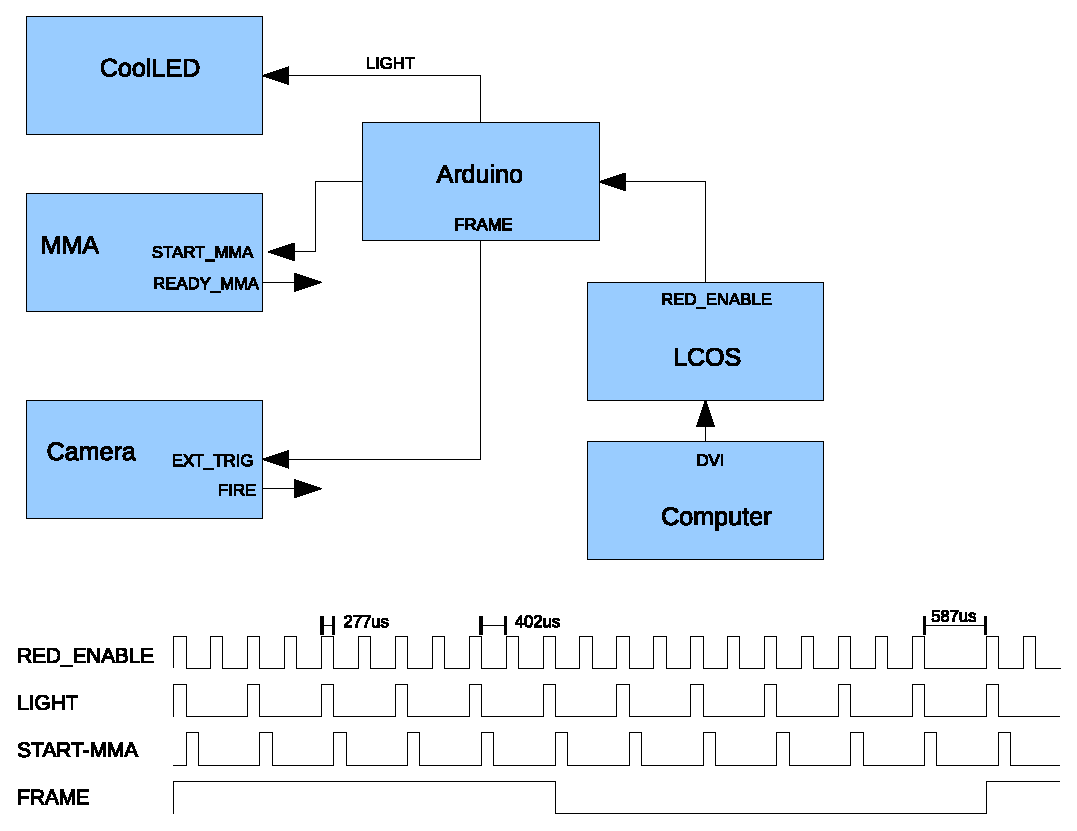
\includegraphics[width=14cm]{../dvi/trigger0}
  \caption{}
  \label{fig:trigger0}
\end{figure}


\begin{figure}[!hbt]
  \centering
  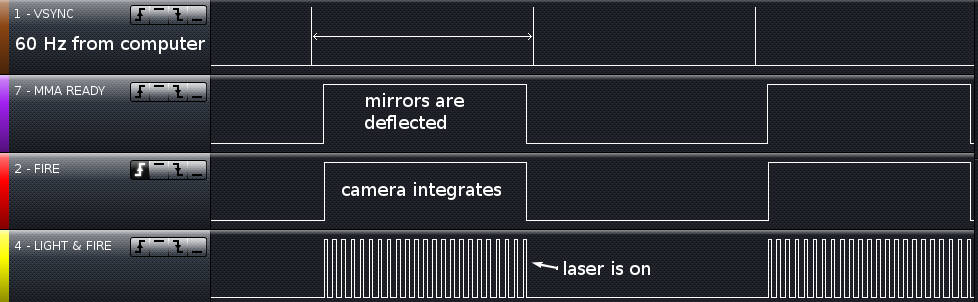
\includegraphics[width=12cm]{screen_logic_labels}
  \caption{Snapshot of the trigger signals with a logic analyzer.}
  \label{fig:screen_logic_labels}
\end{figure}

\begin{figure}[!hbt]
  \centering
  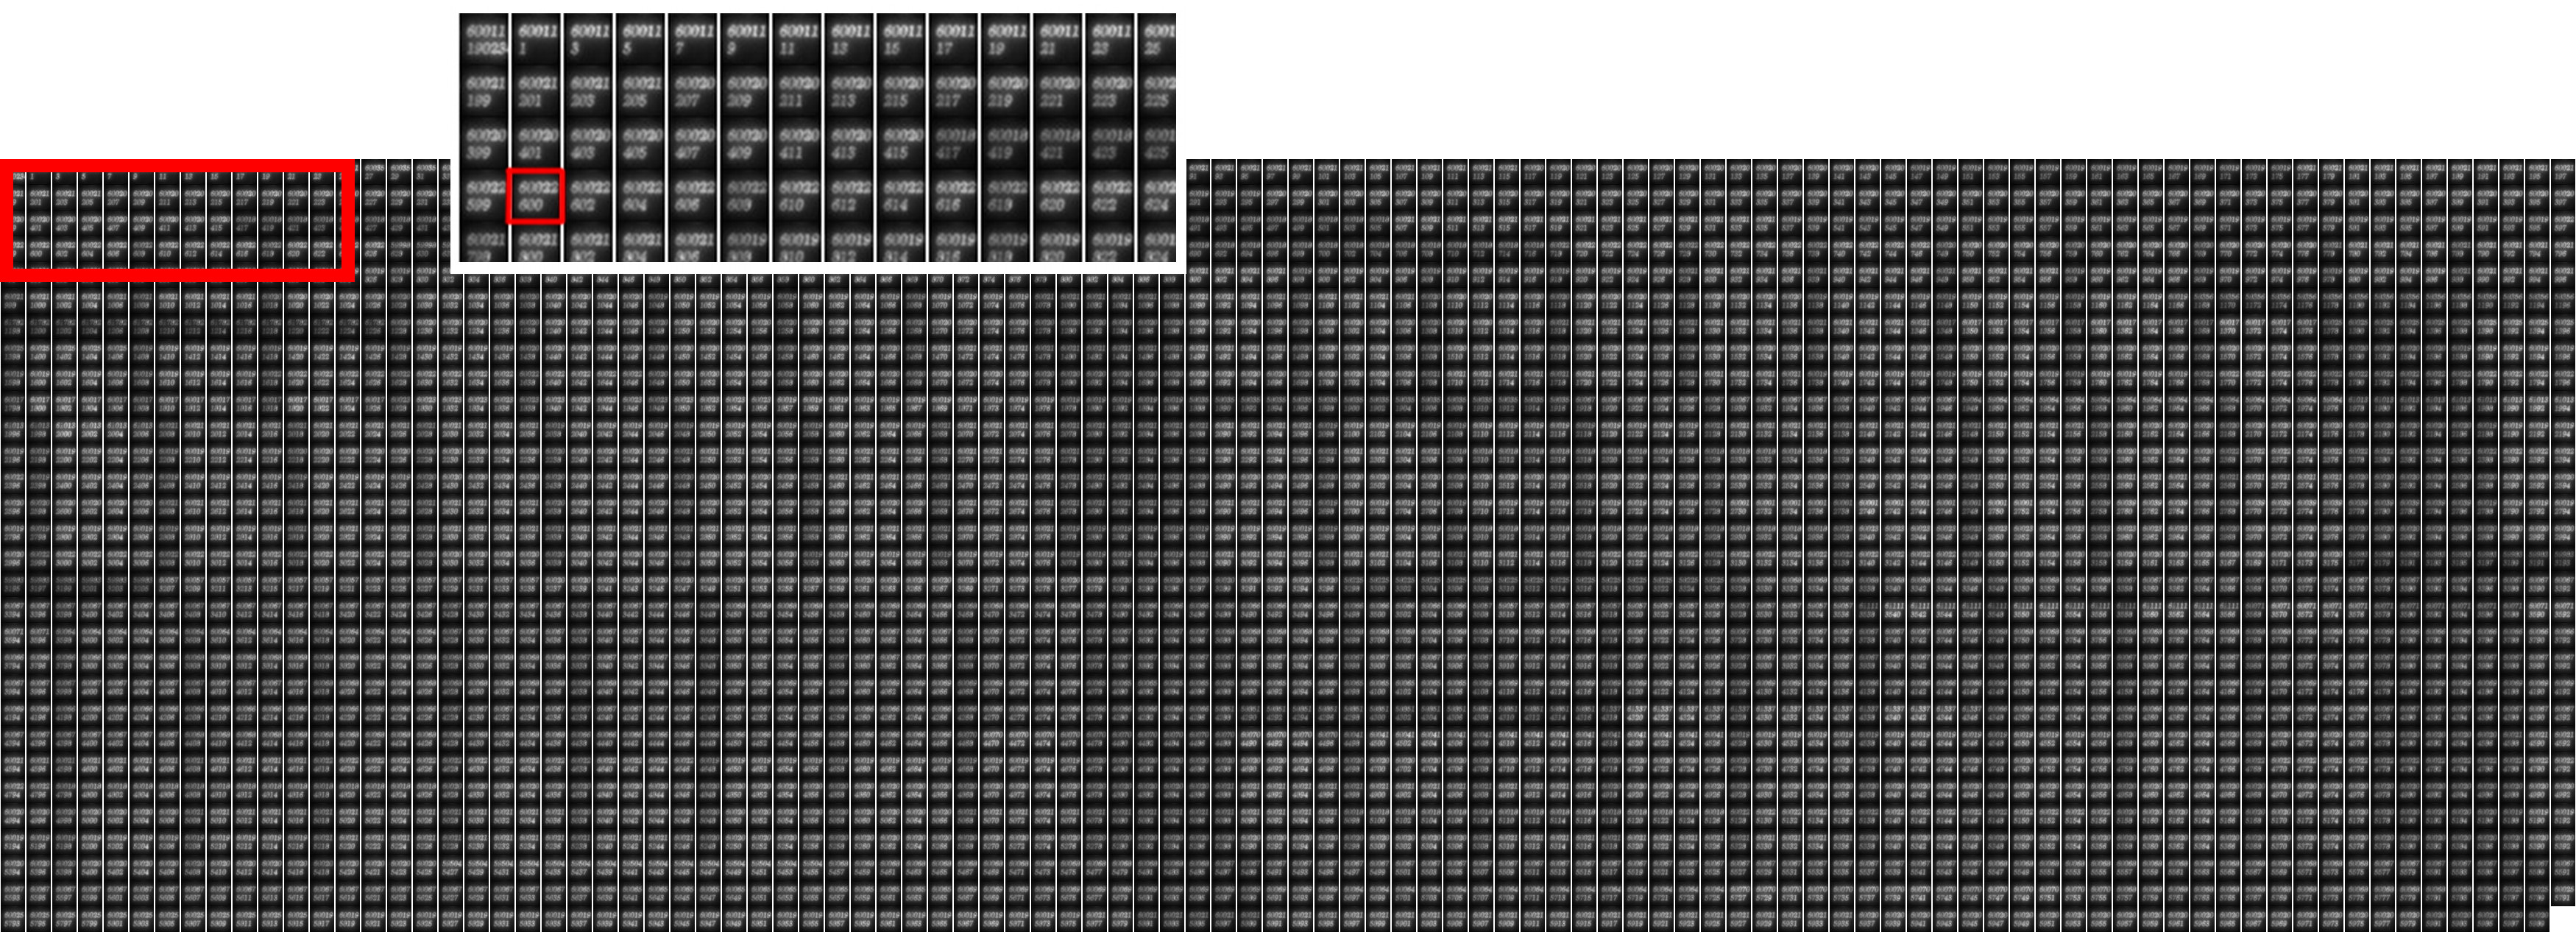
\includegraphics[width=14cm]{fast4-no-first_cut}
  \caption{}
  \label{fig:fast4-no-first_cut}
\end{figure}


\begin{figure}[!hbt]
  \centering
  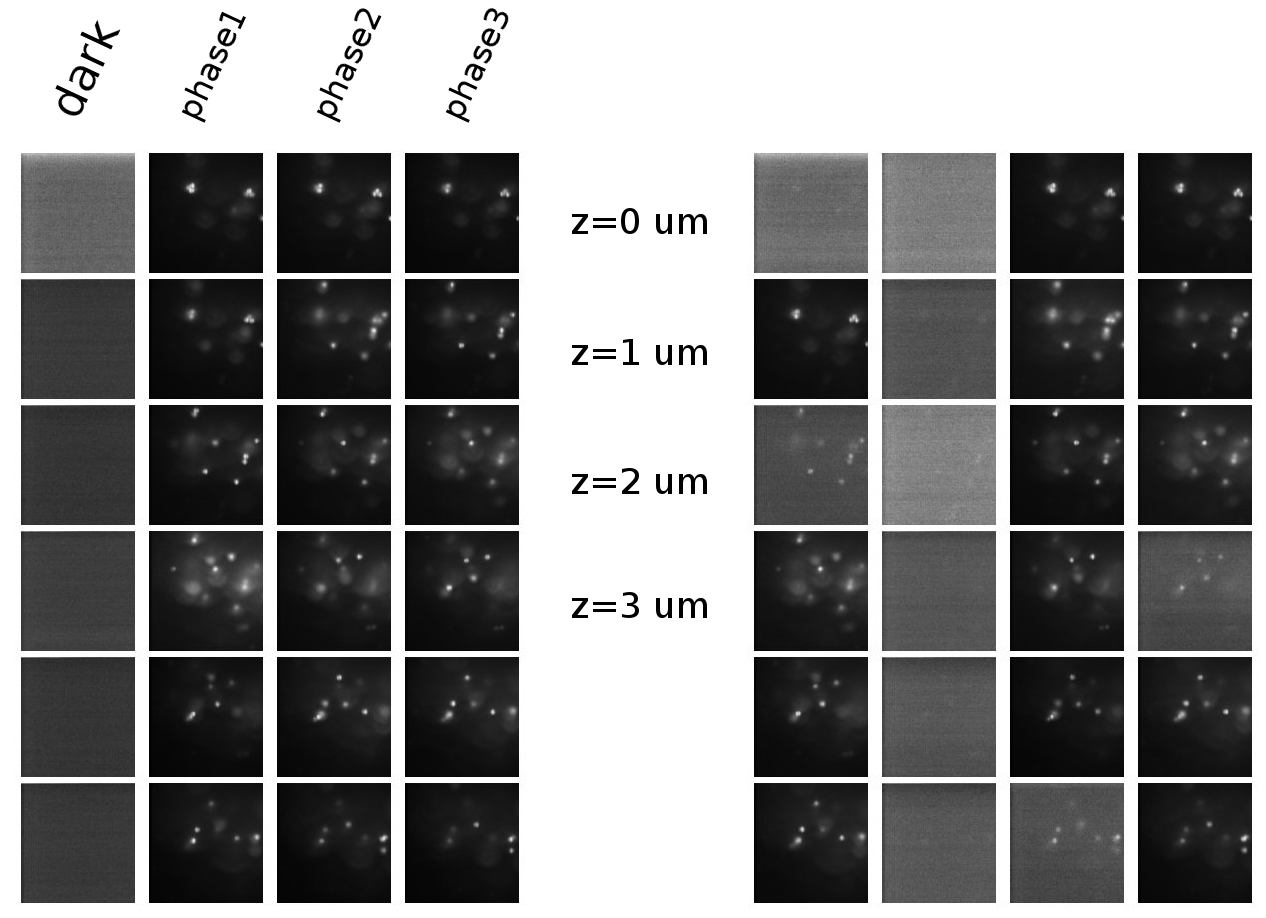
\includegraphics[width=10cm]{dvi-mosaic}
  \caption{{\bf left:} Sequence of images that was aquired while LCoS,
    MMA, z-stage and camera are running in sync. The camera is
    constantly running at \unit[30]{Hz} and the stage moves while a
    black mask is displayed on the MMA as well as the LCoS.}
  \label{fig:dvi-mosaic}
\end{figure}

